\section{Domain Analysis}
\phantomsection

\subsection{Quick Response Codes}
The QR code, which stands for Quick Response Code, is a two-dimensional barcode, which was initially used for tracking inventory. It was developed in Japan by a subdivision of Toyota. Today, it is widely spread and people have found more and more uses for it. The fast gain in popularity was due to the superiority of the QR codes’ read speed and storage capacity versus the UPC barcodes.

The QR code is composed of black square dots placed on a white square background. It is usually read by a phone camera, which has a QR decoding software. The code image is then interpreted and the data is extracted.

The code can be read from any direction in 360 degree. The three corners of the QR code contain the positional detecting patterns, which make this thing possible.

\subsubsection{QR Error Correction}
The QR error correction is used to restore the data on a damaged code. There are four levels of correction. If a higher level is set, the error correction is more efficient but less characters can be encoded. So you must be careful when deciding which error correction level to use. Most of the time, the decisive factor is the environment in which the QR codes will be used. So take the probability of the QR code to be damaged into consideration and decide about the error correction level accordingly.

\subsubsection{QR code sizes}
The black dots in the code are also called modules. Their size are an important factor that categorize the QR codes in readable and not readable by certain devices. The QR codes become unreadable if their modules’ size are below the resolution limitation of the imaging device’s camera.

The QR code is designed in such a way that, the more data you want to store in it, the more columns and rows containing modules will be inserted. Therefore, a QR code must have a bigger size when a larger amount of data is encoded and vice-versa.

So, the QR codes have been categorized in versions, from Version 1 to Version 40.  QR code Versions differing from the previous one by having 4 more modules on each side: Version 1 with ( 21 x 21 modules ) with possibility of storing 25 alphanumerics with the lowest correction level and Version 40 with  ( 177 x 177 modules ) with 1852 alphanumerics. The maximum data storage for each version is derived from the amount of data, character type and correction level.

\begin{figure}[!ht]
\centering
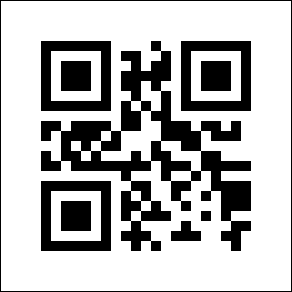
\includegraphics[width=0.3\textwidth,natheight=292, natwidth=292]{qr-v1.png}
\caption{Version 1 QR Code}
\end{figure}


Having this technology at hand, the system gets to simplify the way in which it recognizes the different pages it is processing at the low level of its implementation. Given that information being stored in the QR code will be minimal, it is not required a size bigger than the Version 1 provides us, thus saving some space on the printed paper. The correction level will be set to high, for safety reasons and also because it won’t conflict with the number of characters needed to be encoded.

\clearpage

